\section{Prototyp-Einführung}
In den folgenden Abschnitten wird die Funktionsweise des Prototyps be-schrieben.
Dabei handelt es sich in erster Linie um ein Proof-of-Concept und nicht um eine 
vollumfängliche Softwarelösung. 
Der Prototyp entspricht dabei der im Abschnitt~\ref{section:conclusions} genannten
Lösung mit hierarchisch implementierten Filterregeln, die ankommende Probe-Requests 
in jeder Hierarchiestufe weiter unterteilen. Als Ergebnis entstehen distinkt 
voneinander unterscheidbare Gruppen von Probe-Requests, die potentiell zu einzelnen 
Geräten gehören.

Im Prototyp werden prinzipiell Prozessschritte gemäss folgender Auflistung vorgenommen.
\begin{itemize}
    \item Preprocessing
    \item Vorfilterung
    \item Filterung
\end{itemize}

Bei der Programmierung der Filter wurde darauf geachtet, dass der Input und der Output 
in einem einheitlichen Format gehalten wird. Dieses Vorgehen erlaubt es dem Anwender,
die einzelnen Verfahren in der Reihenfolge auszutauschen und die Ergebnisse untereinander
zu vergleichen und somit eine optimale Reihenfolge festzulegen.
Das gewählte Format ist hierbei ein Python-Dictionary (nachfolgend Dictionary genannt), 
welcher jeweils als Schlüssel-Werte-Paar eine Liste von Bursts beinhaltet.


\subsection{Preprocessing}
Im Preprocessing werden zuerst die einzelnen Probe-Requests aus den JSON-Dateien 
extrahiert und in einzelnen Frame-Klassen instanziert.
Danach werden die Frames anhand der MAC-Adresse in die einzelnen Bursts klassifiziert, 
in Burst-Klassen eingeteilt und als Pyhton-Liste (nachfolgend Liste genannt) gespeichert. 
Die Liste ist dabei aufsteigend nach der Ankunftszeit der Bursts sortiert.
Ein Burst-Objekt hat jeweils die in den Frames verwendete MAC-Adresse, 
die Ankunftszeit des ersten und des letzten Frames, einen Boolean, 
ob das Lokale Bit gesetzt ist und eine Liste von Frames als 
Parameter. Auch die Liste der Frames ist aufsteigend nach der Ankunftszeit der Frames 
sortiert um in weiteren Filterschritten anhand der Ankunftszeit weiter filtern zu können.

\clearpage

\subsection{Vorfilterung}
Die Vorfilterung dient dem Zweck, das Datenset von Bursts zu säubern, die nicht weiter 
gefiltert werden müssen.
Wird in einem Filterforgang festgestellt, dass ein Gerät seine wahre MAC-Adresse 
verwendet, kann diese Adresse in einem Set gespeichert werden und neue ankommende 
Probe-Requests können in der Vorfilterung aus dem Datenset entfernt werden, wenn 
sie eine der MAC-Adressen im Set verwenden. Es können zwei Fälle auftreten, 
in denen Geräte ihre wahre MAC-Adresse verwenden. Erstens, wenn das Gerät seine 
Adresse nicht zufallsgeneriert und zweitens, wenn das Gerät mit einem Acess-Point 
verbunden ist und die randomisierung der MAC-Adresse im verbundenen Zustand
nicht eingestellt hat. Der erste Fall tritt bei älteren Geräten auf, deren 
Betriebssystem eine randomisierung der MAC nicht zulässt oder wenn auf dem Gerät 
die Einstellung, Adressen zufällig zu generieren, nicht eingestellt ist.
Beide Fälle lassen sich daran erkennen, dass ein Gerät über mehrere Bursts hinweg die 
selbe MAC-Adresse verwendet. Es gibt dabei Geräte, die im verbundenen Zustand im SSID-Tag 
die MAC-Adresse des Netzwerks verwenden.

\subsection{Filterung}
Anhand den im Abschnitt~\ref{section:conclusions} genannten Ansätze wurde versucht, 
zwei Filterregeln zu implementierten.
Ziel dieser Filter ist es, Bursts in Gruppen zu unterteilen und diese Gruppen 
so lang weiter zu unterteilen bis potentiell pro Gruppe nur Bursts von einem Gerät 
existieren. 

\subsubsection*{Filtern nach IE-Feldern}
Zuerst werden die Bursts nach den verwendeten Information-Element-Feldern klassifiziert.
In den Messungen wurde festgestellt, dass einzelne Geräte für Probe-Requests merhheitlich
die selben IE-Felder verwenden. 
Die verwendeten IE-Felder werden innerhalb jeder der Listen, 
welche von der Vorfilterung erstellt wurde, 
von Burst zu Burst miteinander verglichen. 
Die Bursts werden dann anhand der IE-Felder in weitere Listen unterteilt und 
zurückgegeben.

\clearpage

\subsection{Verwerfen des Ansatzes zur Zeitbasierten Auswertung
\label{subsection:timefilter}}
Es wurde versucht, das im Unterabschnitt~\ref{subsection:specificapproaches} 
genannte Verfahren für die zeitbasierte Auswertung im Prototypen umzusetzen.
Dabei fiel auf, dass die Dauer eines Bursts (Zeit zwischen dem ersten und 
letzten Frame im Burst) zu kurz ist, um das Verfahren wie geplant anzuwenden.

Selbst Bursts mit mehr als zehn Frames haben eine Dauer von weniger als einer 
Sekunde. Kombiniert mit der unvorhersehbaren Zwischenankunftszeit der Bursts 
ist es unmöglich, ein Zeitfenster zu finden, welches eine genaue Zählung der 
Mobilgeräte ermöglicht.

In einer zusätzlichen Auswertung der Messungen der vier Samsung Galaxy S8 
kann aufgezeigt werden, dass sich selbst identische Gerätetypen mit der 
gleichen Betriebssystemversion sehr unterschiedlich verhalten. 
Das Verhalten wird in der Abbildung~\ref{figure:bursttimeanalysis} dargestellt.

\begin{figure}[h!]
    \centering
    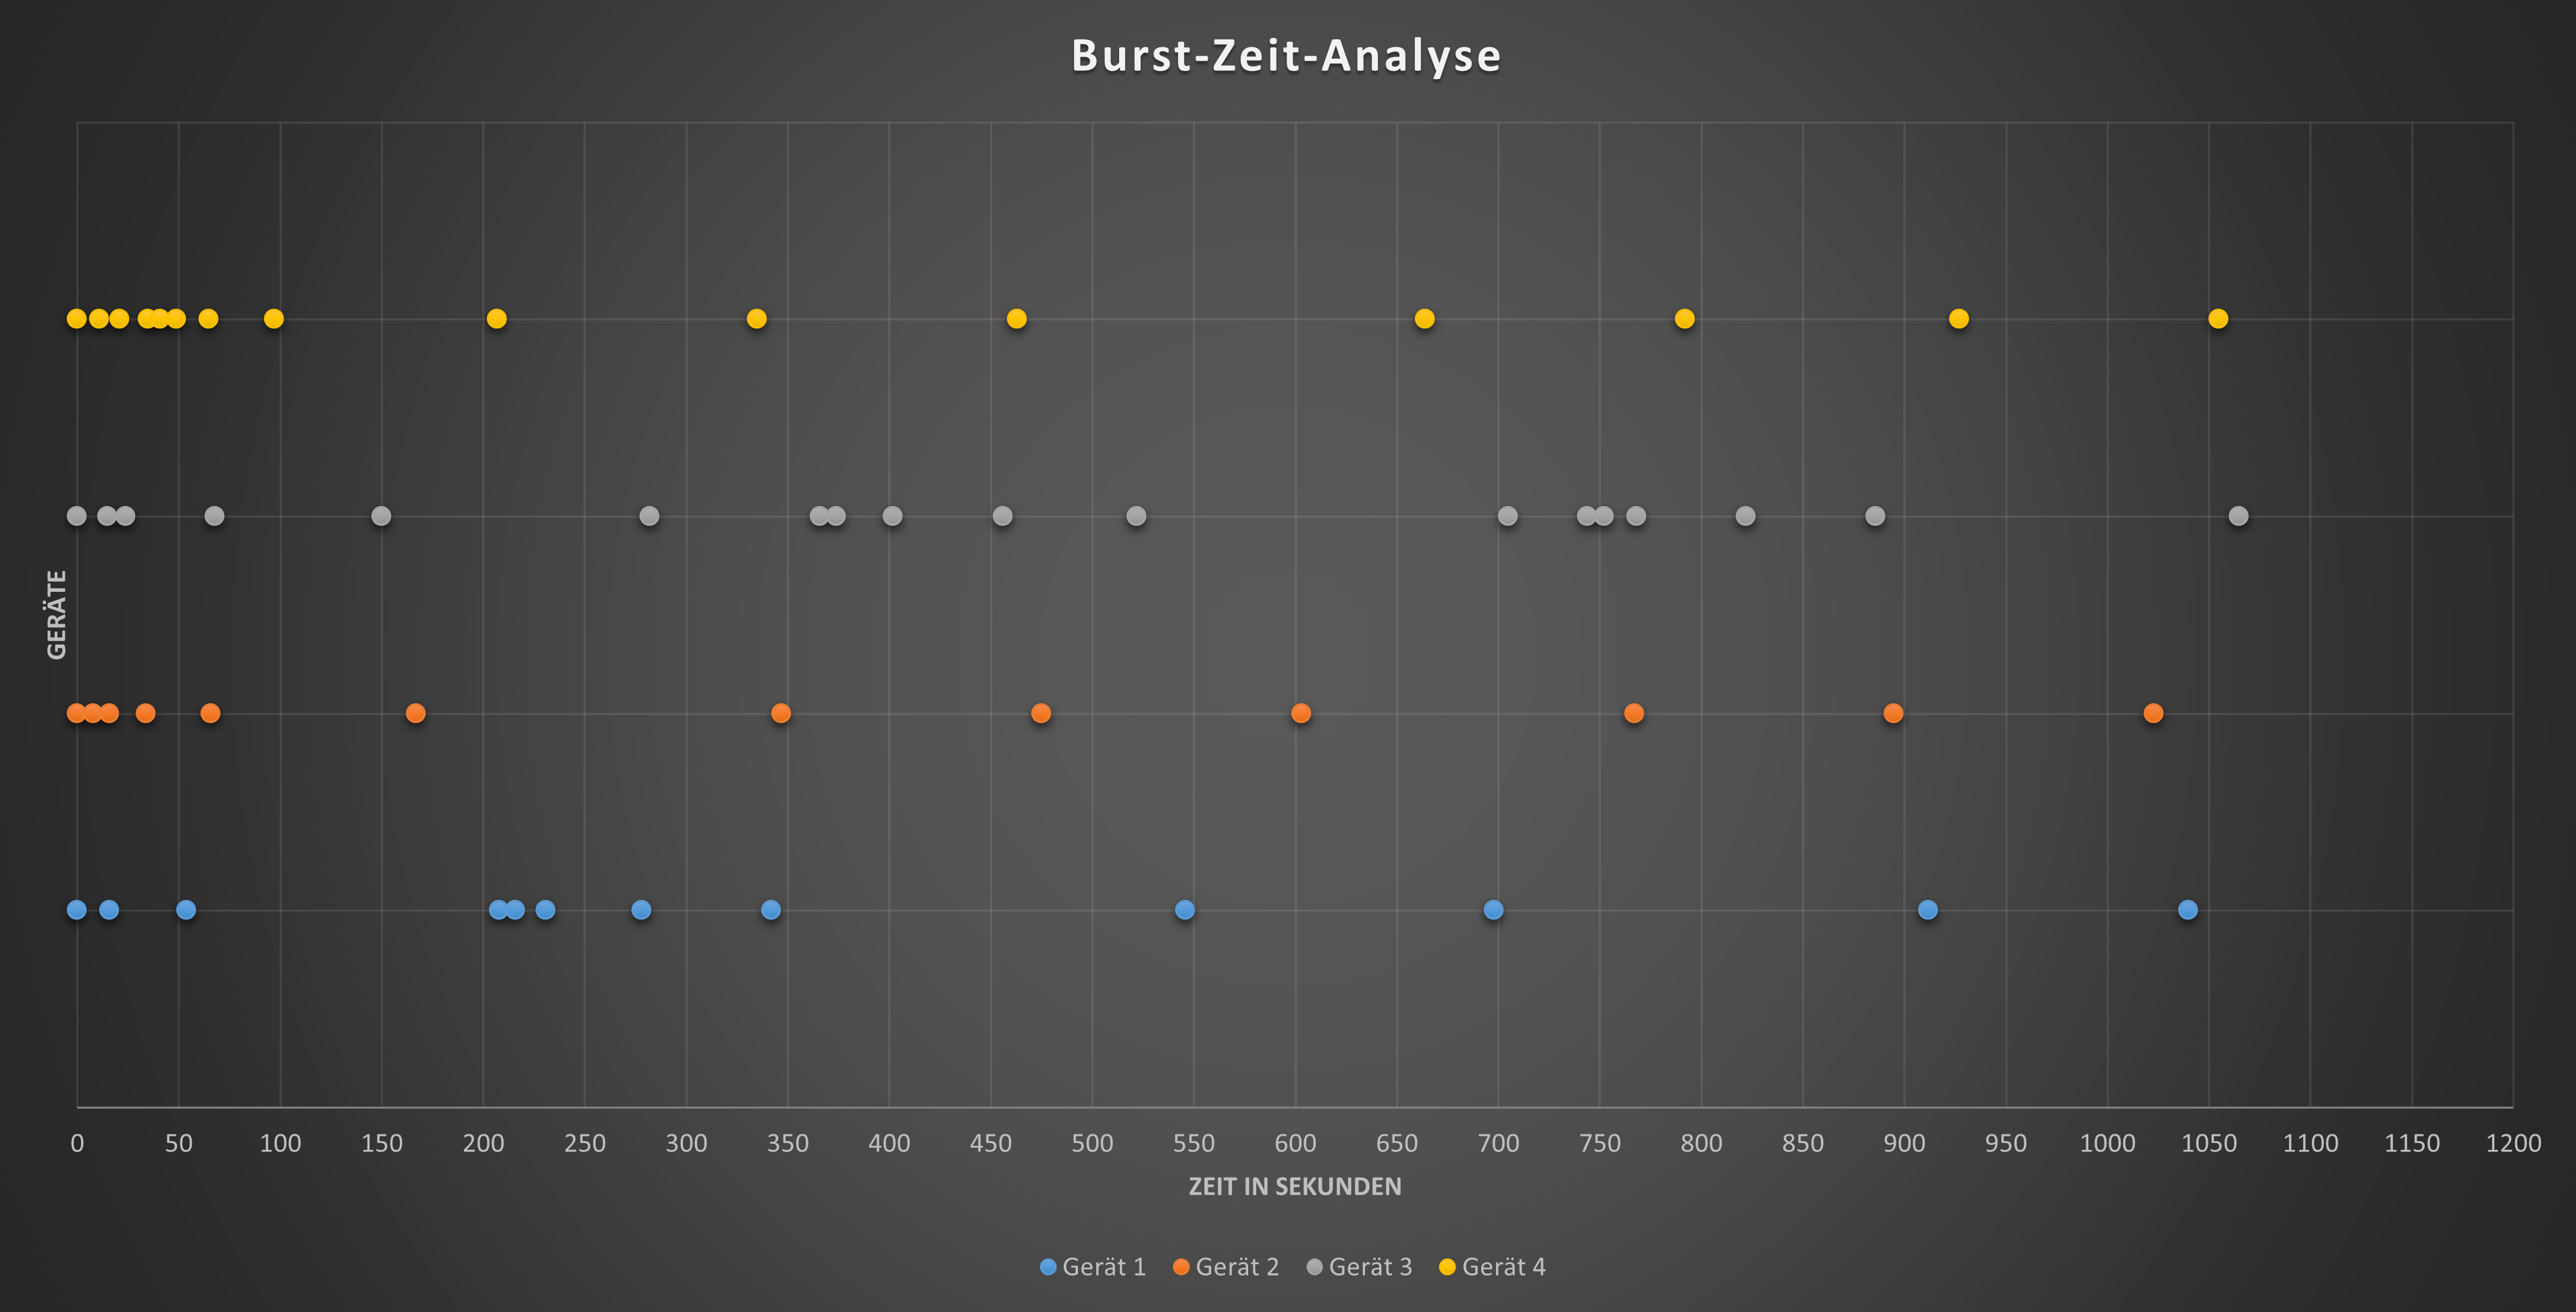
\includegraphics[width=1\linewidth]{Prototype/Burst-Zeit-Analyse.png}
    \caption{Auswertung der Bursts von vier Samsung Galaxy S8 Geräten.
    \label{figure:bursttimeanalysis}}
\end{figure}

Man kann sehr schön erkennen, dass es keine Regelmässigkeit zwischen allen vier 
Geräten gibt. Die Geräte zwei (Orange) und vier (Gelb) verhalten sich ähnlich, 
dadurch dass sie zu Beginn der Messung einige Probe-Requests in kurzer Abfolge 
aussenden und danach die Zwischenankunftszeiten grösser werden.
Das Gerät drei (Grau) scheint die Zwischenankunftszeit der Probe-Requests jeweils 
mit jedem Burst zu erhöhen bis nach ca. 350 Sekunden wieder ein Reset durchgeführt 
wird.
Das Gerät eins (Blau) verhält sich zu Beginn ähnlich wie das Gerät drei, 
wechselt aber zum Zeitpunkt 550 in einen regelmässigen Rithmus.

\clearpage

Wenn man nun als Beispiel den Zeitpunkt 350 betrachtet, kann man sehen, dass 
kurz davor oder danach alle Moblilgeräte Probe-Requests ausgesendet haben. 
Mit einem angenommenen Zeitfenster von 50 Sekunden werden nun alle Bursts 
zwischen den Zeitpunkten 325 und 375 erfasst und es muss entschieden werden,
wie viele Geräte sich im Datenset befinden. Insgesamt werden im Zeitfenster
fünf Bursts erkannt. Jeweils ein Burst gehört zu den Geräten eins, zwei und vier 
und zwei Bursts geören zum Gerät drei. Nun kann dieser Burst aber nicht eindeutig 
zum Gerät drei zugeordet werden, da man nicht sagen kann, ob die zwei Bursts 
zu einem Gerät gehören oder von zwei separaten Geräten ausgesendet wurden ohne
bereits zu wissen, welches Gerät welche Bursts ausgesendet hat.   

\subsection{Konzept: Säuberung des Datensets}
Nachdem die Unterteilungen nach IE-Feldern und Ankunftszeiten vorgenommen wurde, 
kann eine weitere Säuberung vorgenommen werden, indem die Sequenznummern und die 
Local Bits angesehen werden. Die Säuberung des Datensetzs konnte im Prototypen 
aus Zeitgründen nicht umgesetzt werden.

\subsubsection*{Sequenznummern}
Jede Gruppe besteht aus einer Liste von Bursts. Wenn man durch die einzelnen Bursts
iteriert, kann festgestellt werden, ob die Sequenznummern aufsteigend sind, oder ob 
sie pro Burst zufällig generiert werden. Ist nun in der mehrheit der Bursts die 
Sequenznummer aufsteigend und in einem einzelnen Burst nicht, ist die Chance gross,
dass dieser Burst falsch klassifiziert wurde und der Burst kann aus der Liste entfernt
werden. 

\subsubsection*{Local Bit}
In den Experimenten im Abschnitt~\ref{section:androidmeasurements} hat sich herausgestellt,
dass sämtliche Android-Geräte das Local Bit in allen verwendeten MAC-Adressen setzen.
Bei iOS-Geräten wird auch das Local Bit zufallsgeneriert was dazu führt, dass das Bit 
in ca. $50\%$ aller Fälle gesetzt ist.
Da nun iOS-Geräte daran erkannt werden können, dass sie in den IE-Feldern den 
Interworking- und Apple-Vendor-Tag verwenden, kann man in der Liste von Bursts eines 
als Android-Gerät erkannten Geräts diejenigen Bursts entfernen, bei denen das Local Bit 
nicht gesetzt ist.

\clearpage